\documentclass[aspectratio=169,
				xcolor=table]{beamer}
				
% Load general definitions
\usepackage[utf8]{inputenc}
%\usepackage[T1]{fontenc}
\usepackage[brazil]{babel}
\usepackage{amsmath}
\usepackage{amsfonts}
\usepackage{amssymb}
\usepackage{graphicx}
\usepackage{verbatim}
\usepackage{cancel}
\usepackage{askmaps}
\usepackage{tabularx}
\usepackage[table]{xcolor}
%\usepackage{tikz}
\usepackage{multirow}
\usepackage{mathtools}
\usepackage{color, colortbl}
\usepackage{etoolbox}
\usepackage{pbox}
\usepackage{changepage}
\usepackage{xpatch}
\usepackage{array}
\usepackage{marvosym}
\usepackage{tabu}
\usepackage{multicol}
\usepackage{listings}
\usepackage{underscore}
\usepackage{filecontents}
\usepackage[]{algorithm2e}
\usepackage{ragged2e}

\newcolumntype{P}[1]{>{\centering\arraybackslash}m{#1}}
\definecolor{Gray}{gray}{0.75}
\definecolor{Gray2}{gray}{0.85}

\definecolor{lightBlue}{HTML}{DAE8FC}
\definecolor{Blue}{RGB}{51, 51, 204}

%\useinnertheme[lily]{rounded}
\usetheme{UniEvangelica}
%\usetheme{Copenhagen}
%\usetheme{Berlin}
%\usecolortheme{dolphin}
\tolerance=1
\emergencystretch=\maxdimen
\hyphenpenalty=10000
\hbadness=10000

\setbeamertemplate{navigation symbols}{}%remove navigation symbols


\let\olditem=\item% 
\renewcommand{\item}{\olditem \justifying}%
\def\center{\trivlist \centering\item\relax}
\def\endcenter{\endtrivlist}

\setbeamertemplate{itemize/enumerate body begin}{\large}
\setbeamertemplate{itemize/enumerate subbody begin}{\large}

\setbeamertemplate{itemize item}{\raisebox{0.1ex}{$\blacktriangleright$}\hskip0.1em}
\setbeamertemplate{itemize subitem}{\raisebox{0.1ex}{$\blacktriangleright$}\hskip0.1em}

\newcommand{\greenarrow}{\textcolor{green}{\rotatebox[origin=c]{180}{\MVArrowDown}}}

\newcommand{\redarrow}{\textcolor{red}{\MVArrowDown}}

%\newcommand{\ftable}{
%	\begin{table}
%		\large
%		\centering
%		\rowcolors{1}{\ifnumless{\rownum}{2}{Blue}{lightBlue}}{}
%}

\newenvironment{eftable}{
	\begin{table}
		\large
		\centering
		\rowcolors{1}{}{Blue}
		\rowcolors{1}{\ifnumless{\rownum}{2}{Blue}{lightBlue}}{}
	}
	{
	\end{table}
}


%\setbeamertemplate{frametitle}
%{
%	%\vspace*{-2em}	
%	\insertframetitle
%
%	 %\textcolor{white}{\LARGE \insertframetitle}
%
%}

% Specific definitions
\title[]{Arquitetura e Organização de Computadores}
\subtitle[]{Dispositivos de Entrada e Saída}
\author[]{Prof. Alexandre Tannus}
\date{}

\institute[]{\uppercase{Engenharia de Software}}
\title[]{Arquitetura e Organização de Computadores}
\subtitle[]{\uppercase{Dispositivos de Entrada e Saída}}
\author[]{Prof. Alexandre Tannus}
\date{}

\AtBeginSection{\frame{\tableofcontents[currentsection]}}
\setbeamertemplate{frametitle continuation}[from second]

\begin{document}

	\begin{frame}
		\titlepage
	\end{frame}

	\begin{frame}{Objetivos}
		\begin{itemize}
			\item Descrever as características e funções dos dispositivos de entrada e saída (E/S)
			\vspace{1em}
			\item Diferenciar as técnicas de operação de dispositivos de E/S
		\end{itemize}
	\end{frame}

	\begin{frame}{Metodologia}
		\begin{itemize}
			\item O tema da aula é exposto pelo professor em sala de aula. Os alunos interagem durante a apresentação para resolução de dúvidas e exposição de questionamentos relevantes ao tema, os quais podem ser sanados diretamente pelo professor ou serem colocados em discussão pela turma. 
			\vspace{1em}
			\item Ao final da exposição do conteúdo são resolvidos exercícios de fixação, para melhor compreensão do tema. As questões podem ser retiradas de concursos públicos, ENADE, POSCOMP ou de autoria do próprio professor.
		\end{itemize}
	\end{frame}

	\begin{frame}
		\tableofcontents		
	\end{frame}	
	
	\section{Introdução}
	
	\begin{frame}
		\frametitle{Arquitetura de Entrada e Saída}
		\begin{itemize}
			\item Interface do sistema computacional com o mundo exterior
			
		\end{itemize}
		\begin{figure}[hbtp]
		\centering
		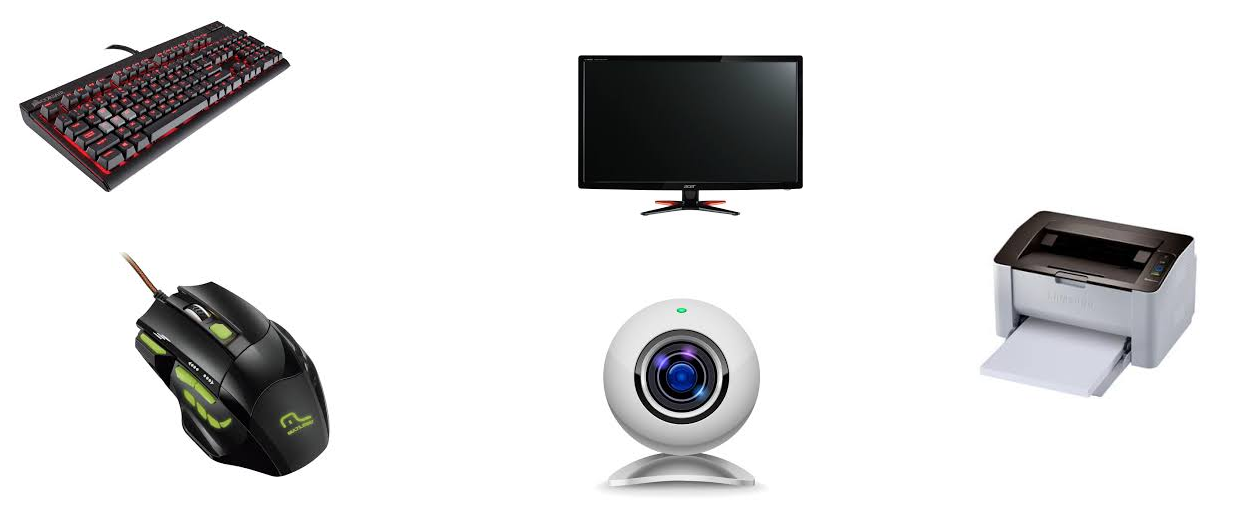
\includegraphics[height=.5\textheight, keepaspectratio]{../figs/cap10/dispositivos.png}
		\end{figure}		
	\end{frame}

	
	\section{Dispositivos de E/S}
	
	\begin{frame}
		\frametitle{Dispositivos de E/S}
		\begin{itemize}
			\item Meio de troca de dados entre o ambiente externo e o computador
			\vspace{1em}
			\item Também conhecidos como \textbf{periféricos}
			\vspace{1em}
			\item Três categorias
			\begin{itemize}
				\item Legíveis ao ser humano
				\item Legíveis à máquina
				\item Comunicação
			\end{itemize}
		\end{itemize}
	\end{frame}
	
	\begin{frame}
		\frametitle{Classificação quanto à transferência de dados}
		\begin{itemize}
			\item Dispositivos de bloco
			\begin{itemize}
				\item Acesso direto 
				\item Sequencial
			\end{itemize}
			\vspace{1em}
			\item Dispositivos de caractere
		\end{itemize}
	\end{frame}
	
	\begin{frame}{Classificação quanto à transferência de dados}
	\begin{eftable}
		\begin{tabular}{|c|c|c|c|}
		\textcolor{white}{Dispositivo} & 
		\textcolor{white}{Entrada/Saída} & 
		\textcolor{white}{Taxa de Dados} & 
		\textcolor{white}{Tipo} \\
		Teclado & Entrada & 100 bps & Caractere \\ 
		Mouse & Entrada & 3800 bps & Caractere \\	 
		Entrada/Saída de voz & Entrada/Saída & 264 kbps & Rajada de blocos	 \\ 
		Entrada de som & Entrada & 3Mbps & Rajada de blocos \\ 
		Scanner & Entrada & 3,2 Mbps & Rajada de blocos \\ 
		Impressora a laser & Saída & 3,2 Mbps & Rajada de blocos \\ 
		Saída de som & Saída & 8Mbps & Rajada de blocos \\ 
		\end{tabular} 	
	\end{eftable}

	\end{frame}

	\begin{frame}{Classificação quanto à transferência de dados}
	\begin{eftable}
		\begin{tabular}{|c|c|c|c|}
		\textcolor{white}{Dispositivo} & 
		\textcolor{white}{Entrada/Saída} & 
		\textcolor{white}{Taxa de Dados} & 
		\textcolor{white}{Tipo} \\
		USB & Entrada ou Saída & 1,6 - 480 Mbps & Rajada de blocos \\ 
		Rede/LAN sem fio & Entrada ou Saída & 11 - 100 Mbps & Rajada de blocos \\ 
		Rede/LAN & Entrada ou Saída & 10 - 1000 Mbps & Rajada de blocos \\ 
		Monitor gráfico & Saída & 800 - 8000 Mbps & Rajada de blocos \\ 
		Disco ótico & Armazenamento & 4 - 400 Mbps & Rajada de blocos \\ 
		Fita magnética & Armazenamento & 29 - 90 Mbps & Rajada de blocos \\ 
		Disco Magnético & Armazenamento & 240 - 3000 Mbps & Rajada de blocos \\ 
		\end{tabular} 	
	\end{eftable}

	\end{frame}	
	
	\begin{frame}
		\frametitle{Interface com módulo de E/S}
		\begin{itemize}
			\item Sinais de controle
			\begin{itemize}
				\item Função que o dispositivo realizará 
			\end{itemize}
			\vspace{.75em}
			\item Sinais de estado
			\begin{itemize}
				\item Estado do dispositivo 
			\end{itemize}
			\vspace{.75em}
			\item Lógica de controle
			\begin{itemize}
				\item Controla a operação do dispositivo
			\end{itemize}
			\vspace{.75em}
			\item Transdutor
			\begin{itemize}
				\item Conversão de dados
				\item Geralmente utiliza \textit{buffers}
			\end{itemize}
		\end{itemize}
	\end{frame}

	\begin{frame}
		\frametitle{Diagrama em blocos de um dispositivo externo (Stallings 2010)}
		\begin{figure}[hbtp]
		\centering
		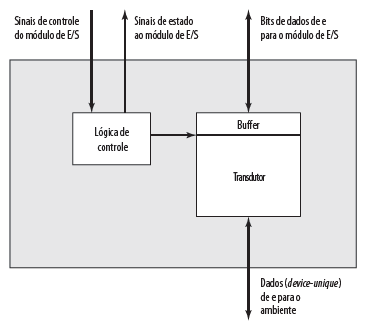
\includegraphics[height=.75\textheight, keepaspectratio]{../figs/cap10/diagrama01.png}
		\end{figure}		
	\end{frame}
	
	\begin{frame}
		\frametitle{Principais dispositivos de E/S}
		\begin{itemize}
		 	\item Teclado
		 	\vspace{1em}
		 	\item Monitor
		 	\vspace{1em}
		 	\item \textit{Mouse}
		 	\vspace{1em}
		 	\item Impressora
		 	\vspace{1em}		 	
		 	\item \textit{Scanner}
		 	
		\end{itemize}
	\end{frame}
	
	\begin{frame}
		\frametitle{Outros dispositivos}
		\begin{figure}[hbtp]
		\centering
		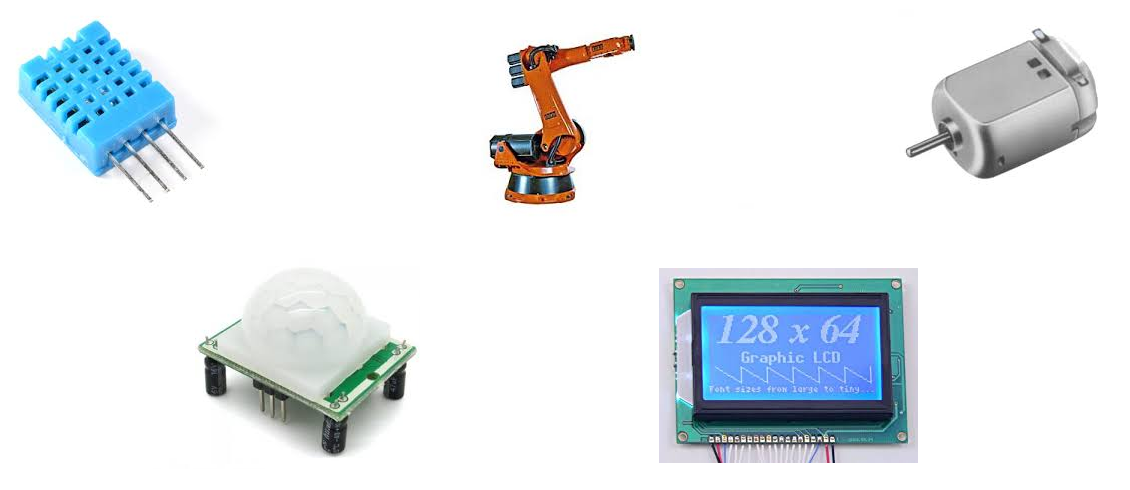
\includegraphics[height=.75\textheight, keepaspectratio]{../figs/cap10/dispositivos2.png}
		\end{figure}		
	\end{frame}

	\section{Módulos de E/S}
	
	\begin{frame}
		\frametitle{Módulos de E/S}
		
		\begin{itemize}
			\item Permite que a CPU visualize, de maneira mais simples, os dispositivos
			\vspace{1em}
			\item Controle do dispositivo
			\vspace{1em}
			\item Dois tipos
			\begin{itemize}
				\item Canal de E/S 
				\item Controlador de E/S
			\end{itemize}
		\end{itemize}
	\end{frame}
	
	\begin{frame}
		\frametitle{Funções do módulo E/S}
		\begin{itemize}
			\item Controle e temporização
			\vspace{1em}
			\item Comunicação com o
			\vspace{1em} processador.
			\item Comunicação com o dispositivo.
			\vspace{1em}
			\item Armazenamento temporário (\textit{buffering}) de dados.
			\vspace{1em}
			\item Detecção de erro
		\end{itemize}
	\end{frame}
	
	\begin{frame}
		\frametitle{Controle e temporização}
		\begin{itemize}
			\item Coordenação do tráfego entre recursos internos e dispositivos externos
			\vspace{1em}
			\item Necessário devido ao compartilhamento de recursos entre diversas atividades
		\end{itemize}
	\end{frame}
	
	\begin{frame}
		\frametitle{Exemplo - Transferência de dados}
		\begin{itemize}
			\item Processador verifica estado do dispositivo de E/S
			\vspace{1em}
			\item Módulo retorna o estado
			\vspace{1em}
			\item Se o dispositivo estiver pronto para transmitir, o processador envia um comando ao módulo de E/S solicitando a transferência
			\vspace{1em}
			\item Módulo obtém os dados do dispositivo externo
			\vspace{1em}
			\item Os dados são transferidos do módulo ao processador
		\end{itemize}
	\end{frame}
	
	\begin{frame}
		\frametitle{Comunicação com o processador}
		\begin{itemize}
			\item Decodificação de comando
			\vspace{1em}
			\item Dados
			\vspace{1em}
			\item Informação de estado
			\vspace{1em}
			\item Reconhecimento de endereço
		\end{itemize}
	\end{frame}
	
	\begin{frame}
		\frametitle{Comunicação com o dispositivo}
		\begin{columns}
			\begin{column}{0.4\textwidth}
				\begin{itemize}
					\item Comandos
					\vspace{1em}
					\item Informação de estado
					\vspace{1em}
					\item Dados				
				\end{itemize}
			\end{column}
			\begin{column}{0.6\textwidth}
				\begin{figure}[hbtp]
				\centering
				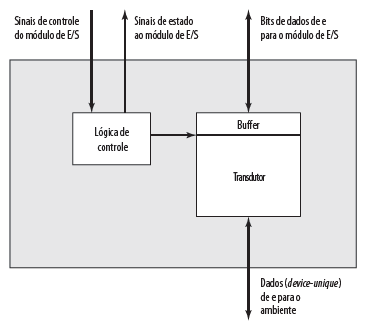
\includegraphics[height=.75\textheight, keepaspectratio]{../figs/cap10/diagrama01.png}
				\end{figure}
			\end{column}
		\end{columns}		
	\end{frame}
	
	\begin{frame}
		\frametitle{\textit{Buffering} de dados}
		\begin{itemize}
			\item Problema de compatibilidade de taxa de transferência (E/S \textit{vs} memória/processador)
			\vspace{1em}
			\item Módulo armazena dados para diminuir quantidade de operações de transferências lentas
			\vspace{1em}
			\item Módulo deve ser capaz de operar nas velocidades do dispositivo e da memória
			
		\end{itemize}
	\end{frame}
	
	\begin{frame}
		\frametitle{\textit{Buffering} de dados}
		
		\begin{figure}[hbtp]
		\centering
		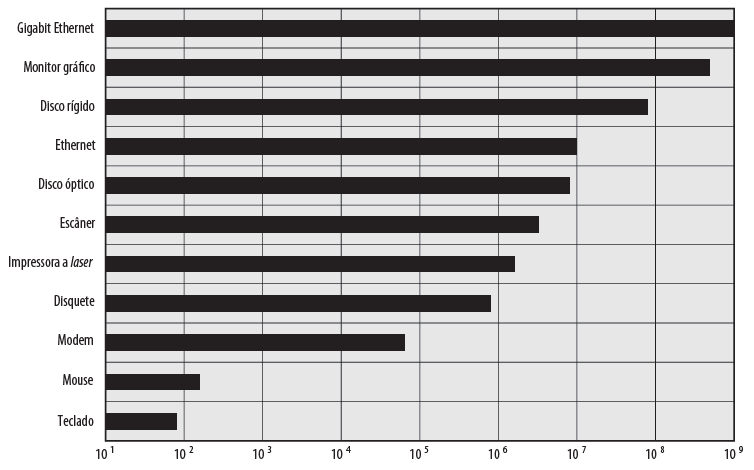
\includegraphics[height=.75\textheight, keepaspectratio]{../figs/cap10/datarate.png}
		\end{figure}
	\end{frame}
	
	\begin{frame}
		\frametitle{Detecção de erro}
		\begin{itemize}
			\item Falhas mecânicas e/ou elétricas
			\vspace{1em}
			\item Alterações em padrões de bits
			\vspace{1em}
			\item Erros de transmissão
		\end{itemize}
	\end{frame}
	
	\begin{frame}
		\frametitle{Questão 1 - DPE-SP 2010}
		A principal função do transdutor em um Módulo de Entrada/Saída do computador é
		\vspace{1em}
		\begin{enumerate}[a]

			\item determinar a função a ser executada pelo dispositivo.
			\item indicar o estado do dispositivo.
			\item armazenar os dados em uma área temporária para serem transferidos.
			\item controlar a operação de um dispositivo.
			\item converter os dados codificados como sinais elétricos para alguma outra forma de energia ou vice-versa.		
		\end{enumerate}
	\end{frame}
	
	\begin{frame}
		\frametitle{Questão 2 - DPE-SP 2010}
		NÃO se trata de uma função de um Módulo de Entrada/ Saída, que faz a interface entre o periférico que ele controla e o barramento do sistema:
		\vspace{1em}
		\begin{enumerate}[a]
			\item Controle e Temporização.
			\item Comunicação com o processador.
			\item Processar cálculos.
			\item Comunicação com dispositivos.
			\item Armazenamento temporário de dados.		
		\end{enumerate}

	\end{frame}	
	
	\begin{frame}
		\frametitle{Questão 3 - Petrobras 2012}
		Qual função dos módulos de E/S está relacionada ao compartilhamento de recursos, tais como o barramento e a memória principal, pelas várias atividades que são realizadas por um sistema?
		\vspace{1em}
		\begin{enumerate}[a]
			\item Armazenamento temporário dos dados
			\item Comunicação com dispositivos
			\item Comunicação com o processador
			\item Detecção de erros 
			\item Temporização		
		\end{enumerate}
	\end{frame}
	
	\section{Endereçamento}	
	\begin{frame}
		\frametitle{Métodos de Endereçamento}
		\begin{itemize}
			\item Mapeado em memória
			\begin{itemize}
				\item – Dispositivo de E/S que partilha o espaço de endereçamento da memória
			\end{itemize}
			\vspace{1em}
			\item E/S isolada
			\begin{itemize}
				\item – Espaço de endereçamento de E/S distinto do espaço de
endereçamento de memória.
			\end{itemize}
		\end{itemize}		
	\end{frame}
	
	\begin{frame}
		\frametitle{Mapeamento em memória}
		\begin{itemize}
			\item Conjunto de endereços reservados da memória
			\vspace{1em}
			\item Utilização de funções comuns de leitura e escrita
			\vspace{1em}
			\item Linhas exclusivas para leitura e escrita
		\end{itemize}
	\end{frame}
	
	\begin{frame}
		\frametitle{E/S isolada}
		\begin{itemize}
			\item Também chamada de mapeamento em E/S
			\vspace{1em}
			\item Espaço de endereçamento independente para dispositivos de E/S
			\vspace{1em}
			\item Portas de E/S acessíveis por operações especiais
			\vspace{1em}
			\item Uma linha de leitura/escrita e outra de entrada/saída
		\end{itemize}
	\end{frame}
	
	\begin{frame}
		\frametitle{Endereçamento - Exemplo}
		\begin{figure}[hbtp]
		\centering
		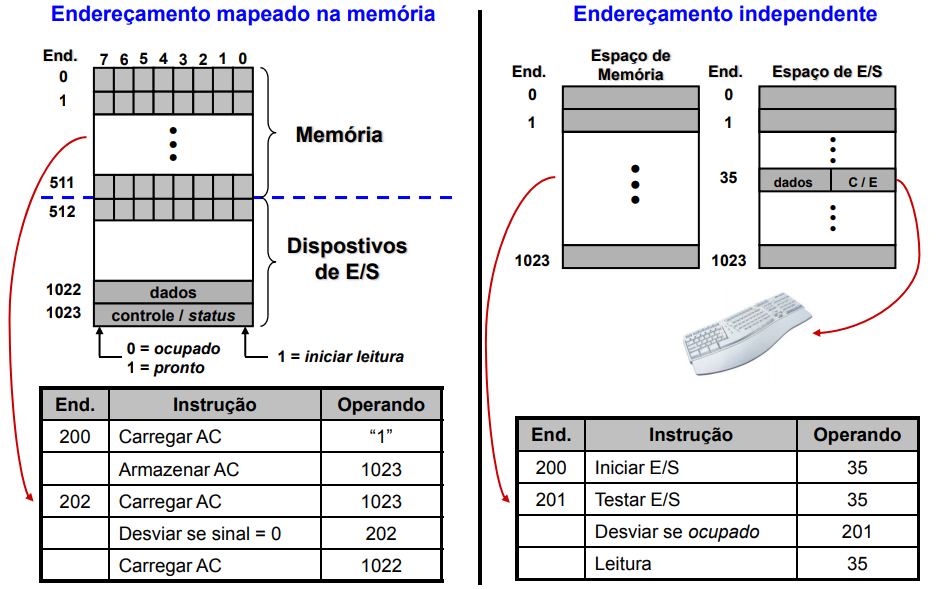
\includegraphics[height=.8\textheight, keepaspectratio]{../figs/cap10/enderecamento.png}
		\end{figure}
		
	\end{frame}

	
	\section{Técnicas}
	
	\begin{frame}
		\frametitle{Técnicas de Operação de E/S}
		\begin{itemize}
			\item Forma como o processador transfere informação entre a memória e os dispositivos periféricos
			\vspace{1em}
			\item Questões fundamentais
			\begin{itemize}
				\item Latência
				\item Taxa de transferência
			\end{itemize}
		\end{itemize}
	\end{frame}
	
	\begin{frame}
		\frametitle{Técnicas de Operação de E/S}
		\begin{itemize}
			\item Programada
			\vspace{1em}
			\item Controlada por interrupção
			\vspace{1em}
			\item Acesso direto à memória (DMA - \textit{Direct Memory Access})
		\end{itemize}
	\end{frame}
	
	\begin{frame}[allowframebreaks]
		\frametitle{Comandos de E/S}
		\begin{itemize}
			\item Controle
			\begin{itemize}
				\item Ativação do periférico e definição da atividade
				\item Comandos específicos para cada tipo de periférico
			\end{itemize}
			\vspace{1em}
			\item Teste
			\begin{itemize}
				\item Verifica condições de estado do módulo e dos periféricos
				\item Ligado/desligado
				\item Condição atual (livre/ocupado)
				\item Detecção de erros
			\end{itemize}
			\framebreak
			\item Leitura
			\begin{itemize}
				\item Módulo obtém dados do periférico
				\item Armazenamento em \textit{buffer}
				\item Possibilidade de solicitação do processador (via barramento de dados)
			\end{itemize}
			\vspace{1em}
			\item Escrita
			\begin{itemize}
				\item Módulo obtém dados no barramento e transmite ao periférico
			\end{itemize}
		\end{itemize}
	\end{frame}
	
	\begin{frame}
		\frametitle{E/S programada}
		\begin{columns}
			\begin{column}{0.7\textwidth}
				\begin{itemize}
					\item Dados trocados entre processador e módulo de E/S
					\vspace{1em}
					\item Controle direto do processador sobre a operação de E/S
					\vspace{1em}
					\item Espera ocupada
				\end{itemize}			
			\end{column}
			\begin{column}{0.3\textwidth}
				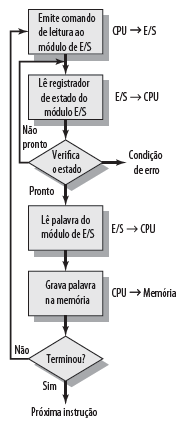
\includegraphics[height=.7\textheight, keepaspectratio]{../figs/cap10/programada.png} 
			\end{column}
		\end{columns}

	\end{frame}
	
	\begin{frame}[allowframebreaks]
		\frametitle{Funcionamento da E/S programada}
		\begin{enumerate}
			\item O hospedeiro lê repetidamente o bit \textit{busy} até que ele seja desligado.
			\vspace{1em}
			\item O hospedeiro liga o bit \textit{write} no registrador \textit{command} e grava um byte no registrador \textit{data-out}.
			\vspace{1em}
			\item O hospedeiro liga o bit \textit{command-ready}.
			\framebreak
			\item Quando o controlador nota que o bit \textit{command-ready} está ligado, ele liga o bit busy.
			\vspace{1em}
			\item O controlador lê o registrador \textit{command} e vê o comando \textit{write}. Ele lê o registrador \textit{data-out} para obter o byte e executa o I/O para o dispositivo.
			\vspace{1em}
			\item O controlador desliga o bit \textit{command-ready}, desliga o bit \textit{error} no registrador de status para indicar que o I/O do dispositivo foi bem-sucedido, e desliga o bit \textit{busy} para indicar que terminou. 
		\end{enumerate}
	\end{frame}

	
	\begin{frame}
		\frametitle{E/S controlada por interrupção}
		\begin{itemize}
			\item Controlador notifica a CPU no momento em que estiver apto para o serviço			
			\vspace{1em}
			\item Elimina a necessidade de \textit{polling}
			\vspace{1em}
			\item Linha de solicitação de interrupção
			\begin{itemize}
				\item CPU examina após a execução de cada instrução
			\end{itemize}
			\vspace{1em}
			\item Manipulação de eventos assíncronos
		\end{itemize}
	\end{frame}
	
	\begin{frame}
		\frametitle{Funcionamento}
		\begin{figure}[hbtp]
		\centering
		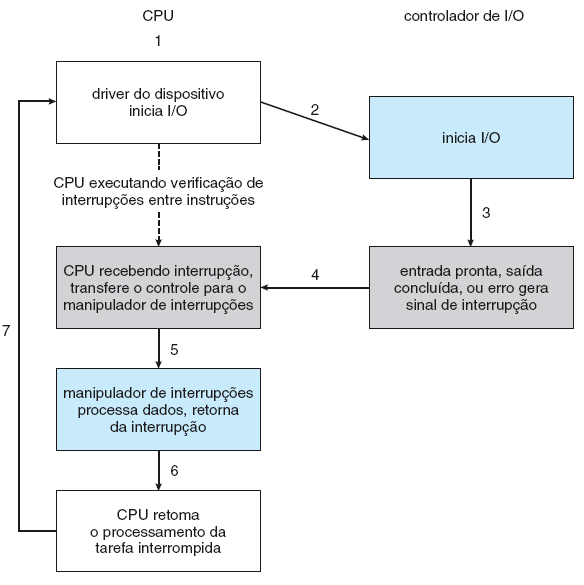
\includegraphics[height=.8\textheight, keepaspectratio]{../figs/cap10/interrupt.png}
		\end{figure}
		
	\end{frame}
	
	\begin{frame}
		\frametitle{Linhas de interrupção}
		\begin{itemize}
			\item Não mascarável
			\begin{itemize}
				\item Reservada para eventos específicos
				\item Obrigatória a execução
			\end{itemize}
			\vspace{1em}
			\item Mascarável
			\begin{itemize}
				\item CPU decide sobre ativação ou inibição
				\item Utilizada pelos controladores para solicitar serviço
			\end{itemize}
		\end{itemize}
	\end{frame}
	
	\begin{frame}
		\frametitle{Recursos de manipulação de interrupções}
		\begin{itemize}
			\item Retardo durante processamento crítico
			\vspace{1em}
			\item Conhecimento do dispositivo que solicitou a interrupção (evitar verificação de todos os periféricos)
			\vspace{1em}
			\item Definição de prioridades
		\end{itemize}
	\end{frame}
	
	\begin{frame}[allowframebreaks]
		\frametitle{Identificação do dispositivo}
		\begin{itemize}
			\item Múltiplas linhas de interrupção
			\begin{itemize}
				\item Impraticável
			\end{itemize}
			\vspace{1em}
			\item Verificação por software
			\begin{itemize}
				\item Rotina de tratamento de interrupção 
				\item Processador verifica cada módulo até encontrar aquele que solicitou a interrupção
				\item Lento
			\end{itemize}
			\framebreak
			\item \textit{Daisy chain}
			\begin{itemize}
				\item Verificação via \textit{hardware}
				\item Linha de requisição comum estruturada em cadeia circular
				\item Utilização de vetor de interrupções (ponteiro para rotina de serviço)				
			\end{itemize}
			\vspace{1em}
			\item Arbitração de barramento 
			\begin{itemize}
				\item Módulo precisa obter controle do barramento
				\item Apenas um módulo pode ativar a linha de interrupção
				\item Utiliza vetor de interrupção
			\end{itemize}
		\end{itemize}
	\end{frame}
	
	\begin{frame}
		\frametitle{E/S por Acesso Direto à Memória}
		\begin{itemize}
			\item DMA (\textit{Direct Memory Access})
			\vspace{1em}
			\item Transferência direta dos dados entre o módulo de E/S e a memória
			\begin{itemize}
				\item Eficiente para periféricos com grande volume de transferência de dados (dispositivos de armazenamento)				
			\end{itemize}
			\vspace{1em}
			\item Utiliza \textit{hardware} específico - controlador de DMA
		\end{itemize}
	\end{frame}
	
	\begin{frame}[allowframebreaks]
		\frametitle{Funcionamento}
		\begin{enumerate}
			\item Driver do dispositvo é solicitado a transferir dados para o \textit{buffer} no endereço X 
			\vspace{1em}
			\item Driver do dispositivo solicita ao controlador do disco para transferir C bytes do disco para o buffer no endereço X
			\vspace{1em}
			\item Controlador do disco inicia transferência DMA
			\framebreak
			\item Controlador do disco envia cada byte ao controlador de DMA
			\vspace{1em}
			\item Controlador de DMA transfere bytes para  buffer X, aumentando o endereço e diminuindo C até $C=0$
			\vspace{1em}
			\item Quando $C=0$, o DMA interrompe a CPU para sinalizar a conclusão da transferência
		\end{enumerate}
	\end{frame}
	
	\begin{frame}[allowframebreaks]
		\frametitle{Modos de transferência}
		\begin{itemize}
			\item Em bloco (contínuo)
			\begin{itemize}
				\item Toda a transferência é realizada de uma só vez
				\item Adequado apenas quando todos os dados já estão disponíveis
			\end{itemize}
			\vspace{1em}
			\item A pedido (em rajada)
			\begin{itemize}
				\item Limite de dados 
				\item Adequado para periféricos que produzem e transferem dados ao mesmo tempo (ex: placas de vídeo)
			\end{itemize}
			\framebreak
			\item Palavra a palavra (simples)
			\begin{itemize}
				\item Transfere palavras isoladas
				\item Possibilidade de execução de instruções pela CPU entre as transferências de DMA
			\end{itemize}
		\end{itemize}
	\end{frame}
	
	\begin{frame}
		\frametitle{Roubo de ciclos (Cycle stealing)}
		\begin{itemize}
			\item Uso da CPU entre as transferências de DMA
			\vspace{1em}
			\item Impossibilidade do processador realizar acesso à memória
			\vspace{1em}
			\item Otimização
			\begin{itemize}
				\item Controlador de DMA acessar o barramento apenas em ciclos em que o processador não acessa a memória
				\item Impacto na velocidade de transferência
			\end{itemize}
		\end{itemize}
	\end{frame}
	
	\begin{frame}
		\frametitle{Comparação de técnicas}
		\begin{figure}[hbtp]
		\centering
		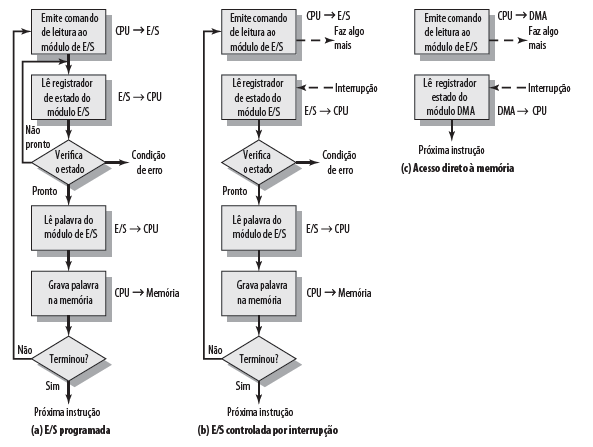
\includegraphics[height=.8\textheight,keepaspectratio]{../figs/cap10/tecnicas.png}
		\end{figure}		
	\end{frame}

	\begin{frame}
		\frametitle{Comparação de técnicas}
		\begin{eftable}
			\centering
			\begin{tabular}{ccc}
			{\color[HTML]{FFFFFF} Característica}                                      & {\color[HTML]{FFFFFF} \begin{tabular}[c]{@{}c@{}}Processador \\ livre\end{tabular}} & {\color[HTML]{FFFFFF} \begin{tabular}[c]{@{}c@{}}Processador \\ ocupado\end{tabular}} \\
			\begin{tabular}[c]{@{}c@{}}Sem envolvimento \\ do processador\end{tabular} & \begin{tabular}[c]{@{}c@{}}Acesso direeto à \\ memória (DMA)\end{tabular}           &                                                                                       \\
			\begin{tabular}[c]{@{}c@{}}Processador \\ controla E/S\end{tabular}        & \begin{tabular}[c]{@{}c@{}}E/S controlada \\ por interrupção\end{tabular}           & \begin{tabular}[c]{@{}c@{}}E/S  \\ programada\end{tabular}
			\end{tabular}
		\end{eftable}			
	\end{frame}

	\begin{frame}
		\frametitle{Questão 4 - UNIFESP 2009}
		Acerca de Módulo de Entrada e Saída Programada, marque a alternativa CORRETA: 
		\begin{enumerate}[a]
			\item Nela, a CPU tem controle indireto da operação de Entrada e Saída.
			\item Nela, a CPU indica que as entradas e saídas programadas sejam cronometradas digitalmente para evitar atrasos no controle dos processos.
			\item Nela, a CPU aguarda até que a operação de Entrada e Saída enviada seja finalizada.
			\item Nela, a finalização é indicada pela mudança dos bytes de situação do módulo de Entrada e Saída, que é consultada pela CPU.		
		\end{enumerate}
	\end{frame}	
	
	\begin{frame}
		\frametitle{Questão 5 - UFG 2017}
		A adoção de um mecanismo de E/S orientada à interrupção tem como desvantagem a ocorrência de uma interrupção para cada caractere, o que desperdiça uma certa quantidade de tempo de CPU. Uma solução, em geral, mais eficiente para realizar E/S é usar
		\vspace{1em}
		\begin{enumerate}[a]
			\item o sistema de \textit{spooling}. 
			\item a E/S programada. 
			\item o acesso direto à memória.
			\item a técnica de \textit{polling}.		
		\end{enumerate}
	\end{frame}
	
	\begin{frame}
		\frametitle{Questão 6 - IF-PA 2016}
		Em um computador, o módulo de E/S (Entrada/Saída) é responsável por coordenar o acesso aos recursos de processamento da CPU. Com relação a este assunto, afirma-se que
		\vspace{1em}
		\begin{enumerate}[I]
			\item Na técnica de E/S programada o processador implementa um loop de interrogação, para verificar quando o dispositivo estará pronto para outra tarefa. Enquanto isso, o processador não pode realizar outras atividades.
			\item Na técnica de E/S por interrupção é o dispositivo ou o periférico que sinaliza ao processador, por meio de interrupção, quando estiver pronto.
			\item O método de E/S que utiliza mais recursos do processador nas interrogações do estado do dispositivo é a DMA (Acesso Direto a Memória).		
		\end{enumerate}
	\end{frame}
	
	\begin{frame}
		\frametitle{Questão 7 - UFPA 2017}
		Sobre dispositivos de entrada e saída, considere as afirmativas abaixo:
		\vspace{1em}
		\begin{enumerate}[I]
			\item Barramentos não têm protocolos definidos para trocas de mensagens entre os envolvidos.

			\item Interrupções são usadas pelos dispositivos para avisar sobre operações ao sistema operacional.

			\item Todos os dispositivos de entrada e saída são considerados dispositivos de bloco.

			\item DMA (Direct Memory Access – Acesso Direto à Memória) permite que dispositivos acessem a memória do sistema independente da UCP.		
		\end{enumerate}
	\end{frame}
	
	\begin{frame}
		\frametitle{Questão 8 - TRE-MA 2015}
		Referente a E/S, assinale a alternativa INCORRETA:
		\vspace{.5em}
		\begin{enumerate}[a]
			\normalsize
			\item A E/S mapeada em memória é um esquema de E/S em que partes do espaço de endereçamento são atribuídas a dispositivos de E/S e leituras e escritas para estes endereços são interpretadas como comandos aos dispositivos de E/S.
			\item Dentre as técnicas possíveis para interação entre processador e E/S o acesso direto a memória é a menos eficiente pois o módulo DMA vai concorrer com o processador no acesso ao barramento do sistema.
			\item Na E/S programada os dados são trocados entre o processador e o módulo de E/S e quando o processador fornece um comando ao módulo ele deve esperar até que a operação de E/S termine.
			\item O processo de verificar periodicamente o status de um dispositivo de E/S para determinar a necessidade de atender ao dispositivo é denominado \textit{polling}.		
		\end{enumerate}
	\end{frame}

	\begin{frame}{Respostas}
		\begin{itemize}
			\item Questão 1 - E
			\item Questão 2 - C
			\item Questão 3 - E
			\item Questão 4 - C
			\item Questão 5 - C
			\item Questão 6 - I e II estão corretas
			\item Questão 7 - II e IV estão corretas
			\item Questão 8 - B
		
		\end{itemize}
	\end{frame}
			
	\section{Referências}
	\begin{frame}{Bibliografia}
		\nocite{Delgado2017}
		\nocite{Stallings2010}
    	\bibliographystyle{ieeetr}
    	\bibliography{../refs}
    	
	
	\end{frame}

\end{document}